\begin{Exercise}[title=Énergie d'ionisation]
\begin{center}
		\begin{tabular}{|c|c|c|c|c|c|c|c|c|c|c|}
			\hline
			Éléments & Sc &Ti &V &Cr &Mn &Fe &Co &Ni &Cu &Zn \\
			\hline
			$(EI)_d$ \si{\kJ\per\mol}& 454 &538 &610 &694 &765 &837 &909 &969 &1 029 & - \\
			\hline
			$(EI)_s$ \si{\kJ\per\mol}& 550 &586 &610 &534 &658 &682 &706 &730 &741 &906\\
			\hline
	\end{tabular}
\end{center}
Le tableau ci-dessus rassemble les énergies d’ionisation des orbitales atomiques 3d et 4s des atomes gazeux de la première série de transition correspondant aux deux processus
 ci-dessous :
\[3d^x4s^y \to 3d^(x-1) 4s^y + 1e^- ~~ (EI)_d\]
\[3d^x 4s^y \to 3d x 4s^(y-1) + 1e^-\]
(EI: Énergie d'ionisation))
\Question. Montrer que la variation relative des énergies $(EI)_d$ et $(EI)_s$ dans la séquence cobalt-nickel-cuivre traduit un caractère particulier pour ce dernier.
\Question Représenter $\Delta E = [(EI)_s -(EI)_d ]$ en fonction de Z. Donner la signification physique de $\Delta E$.
\Question Montrer que ces données expliquent le non-respect de la règle de Klechkowsky pour les configurations électro-
niques du chrome et du cuivre.

\end{Exercise}
\begin{Answer}
	\Question On constate, pour la ligne des (EI) d une augmentation continue de l’énergie d’ionisation avec Z : les OA s’abaissent lorsque Z augmente. Pour la ligne des (EI) s , on constate grossièrement le même phénomène sauf pour le chrome et pour le cuivre : l’extraction d’un électron de la couche 4s est donc plus aisée pour ces deux atomes traduisant la configuration électronique $[Ar]4s^1 3d^5$ et $[Ar]4s^1 3d^10$ pour le chrome et le cuivre respectivement.
	\Question $\Delta E$ représente l’aptitude à extraire l’électron d’une OA plutôt que d’une autre. En l’occurrence, l’aptitude à extraire un	électron s devant un électron d :
	\begin{center}
		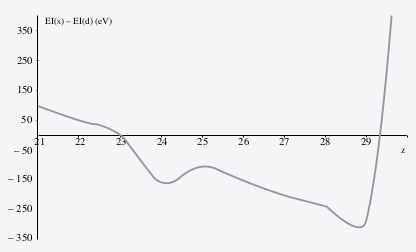
\includegraphics[width=0.4\linewidth]{../fig/Delta_EZ.png}
	\end{center}
	On constate qu’à partir de Z = 23 (vanadium) il est plus facile
	d’extraire un électron s qu’un électron d. Il y a deux cas remarquables : le chrome et le cuivre pour lesquels il est particulièrement facile d’arracher le seul électron s.
	\Question En effet, l’exception de remplissage est expérimentalement mise en évidence, les deux valeurs exceptionnellement basses 	pour Cr et Cu traduit le supplément de stabilité d’une couche $d$ à moitié ou totalement remplie.

\end{Answer}
